\subsection{Supercontinuum light source plots}

\begin{figure}[H]
\begin{subfigure}[h]{0.50\textwidth}
        \centering
        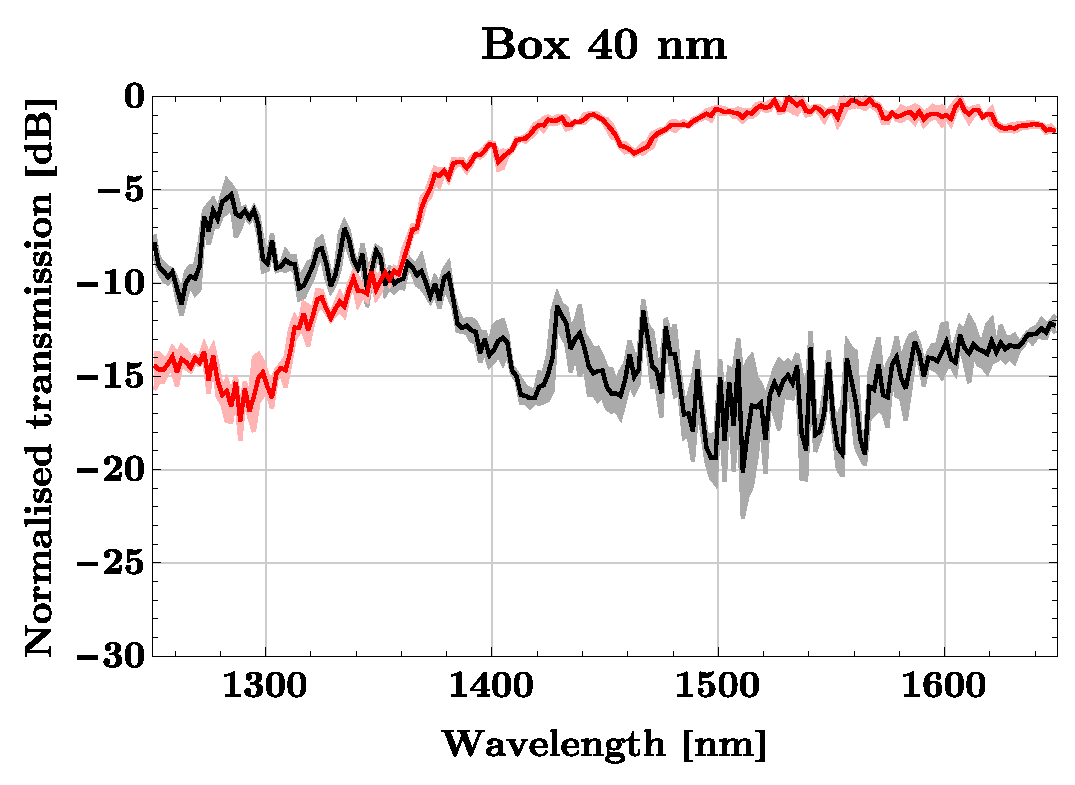
\includegraphics[width=1.0\textwidth]
        {fig/Kilde3Supercontinuum/box40supercontinuum.eps}
        \caption{Transmission through the box structure with feature size 40 nm.}
        \label{fig:transmissionkilde3_a}
    \end{subfigure}%
    ~ 
    \begin{subfigure}[h]{0.50\textwidth}
        \centering
        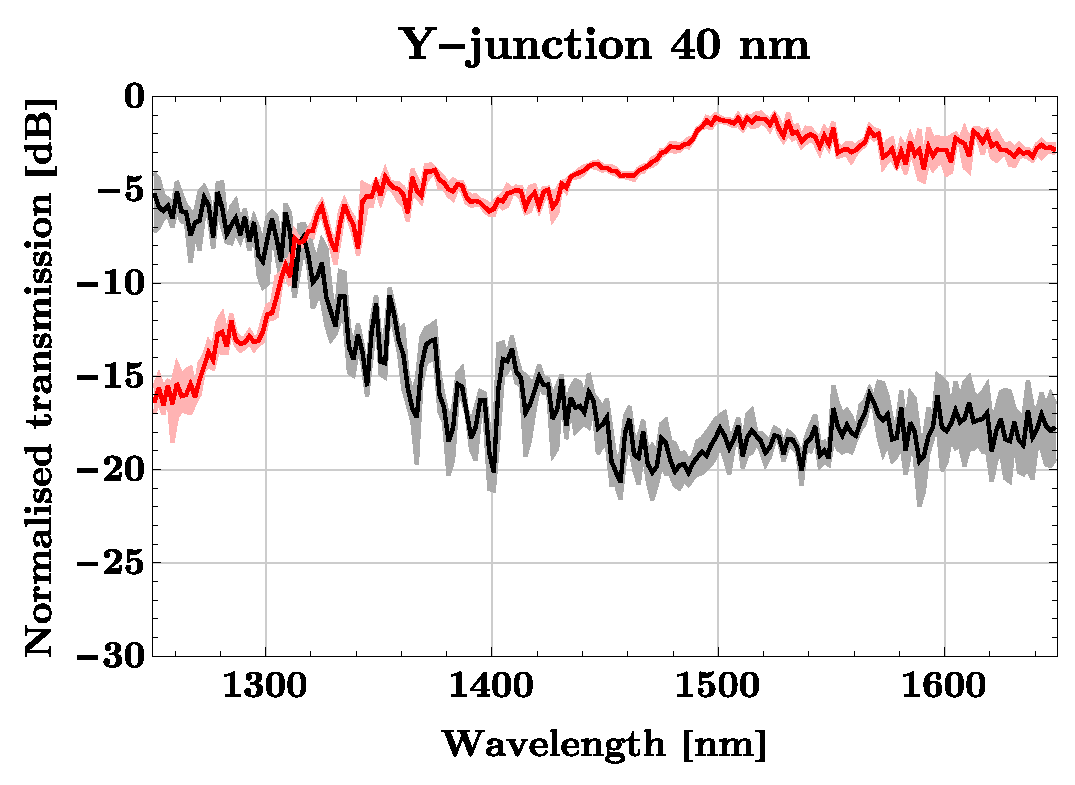
\includegraphics[width=1.0\textwidth]
        {fig/Kilde3Supercontinuum/yjunc40supercontinuum.eps}
        \caption{Transmission through the Y-junction structure with feature size 40 nm.}
        \label{fig:transmissionkilde3_b}
    \end{subfigure}
    
    \vspace{5 mm}
    
    
    \begin{subfigure}[h]{0.50\textwidth}
        \centering
        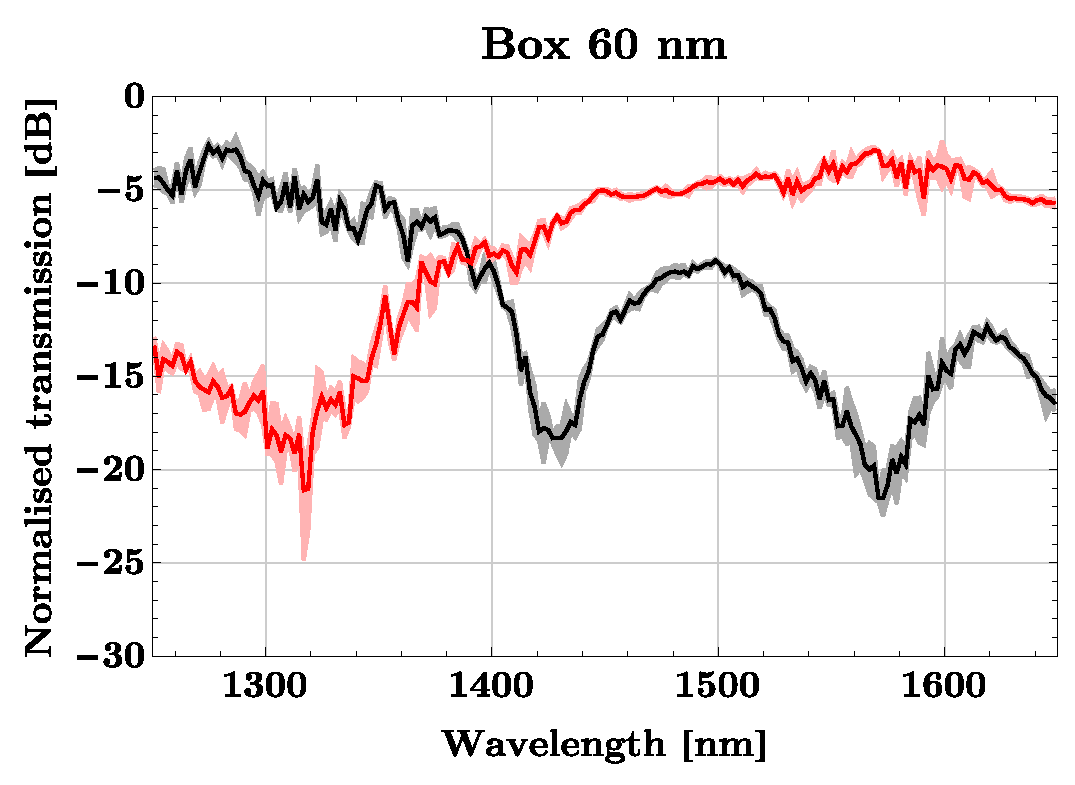
\includegraphics[width=1.0\textwidth]
        {fig/Kilde3Supercontinuum/box60supercontinuum.eps}
        \caption{Transmission through the box structure with feature size 60 nm.}
    \end{subfigure}%
    ~ 
    \begin{subfigure}[h]{0.50\textwidth}
        \centering
        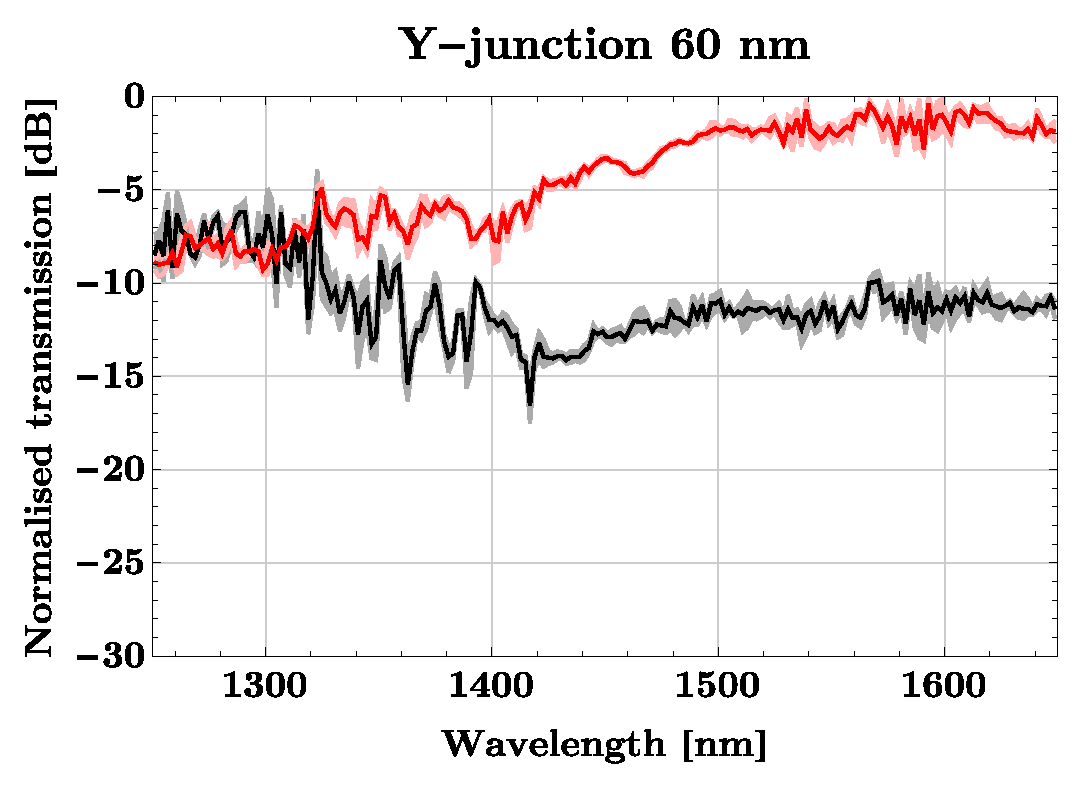
\includegraphics[width=1.0\textwidth]
        {fig/Kilde3Supercontinuum/yjunc60supercontinuum.eps}
        \caption{Transmission through the Y-junction structure with feature size 60 nm.}
    \end{subfigure}
    
    \vspace{5 mm}
    
    \begin{subfigure}[h]{0.5\textwidth}
        \centering
        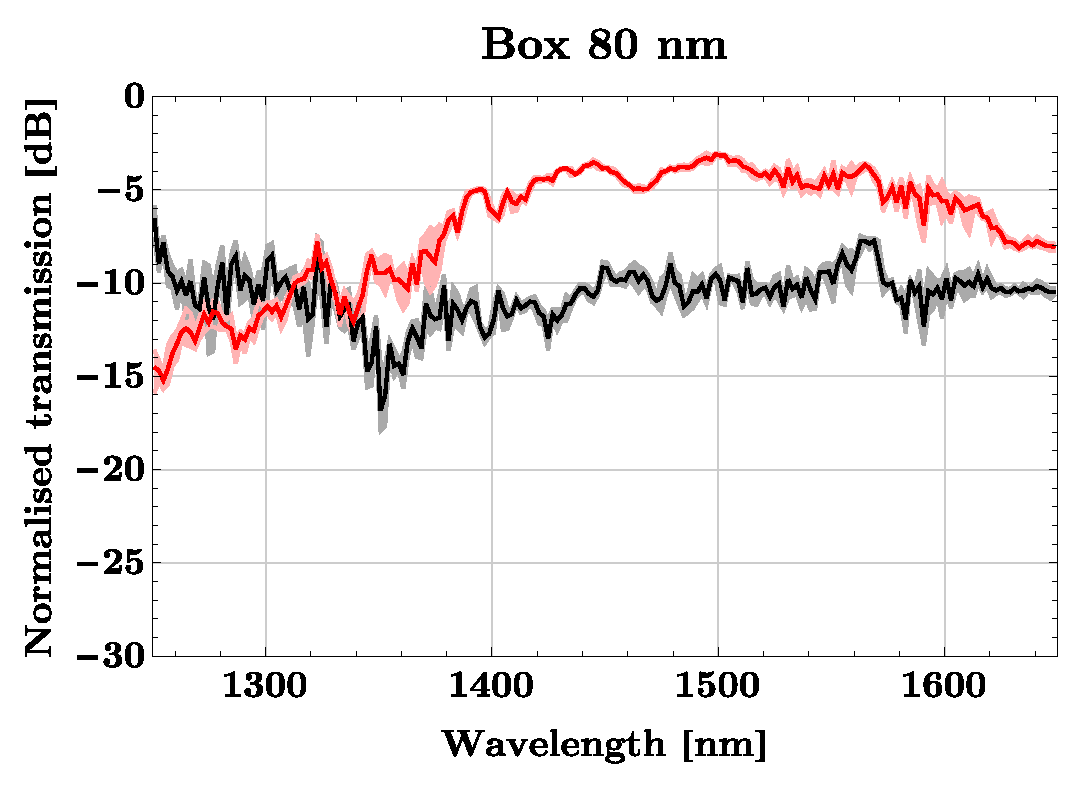
\includegraphics[width=1.0\textwidth]
        {fig/Kilde3Supercontinuum/box80supercontinuum.eps}
        \caption{Transmission through the box structure with feature size 80 nm.}
    \end{subfigure}%
    ~ 
    \begin{subfigure}[h]{0.50\textwidth}
        \centering
        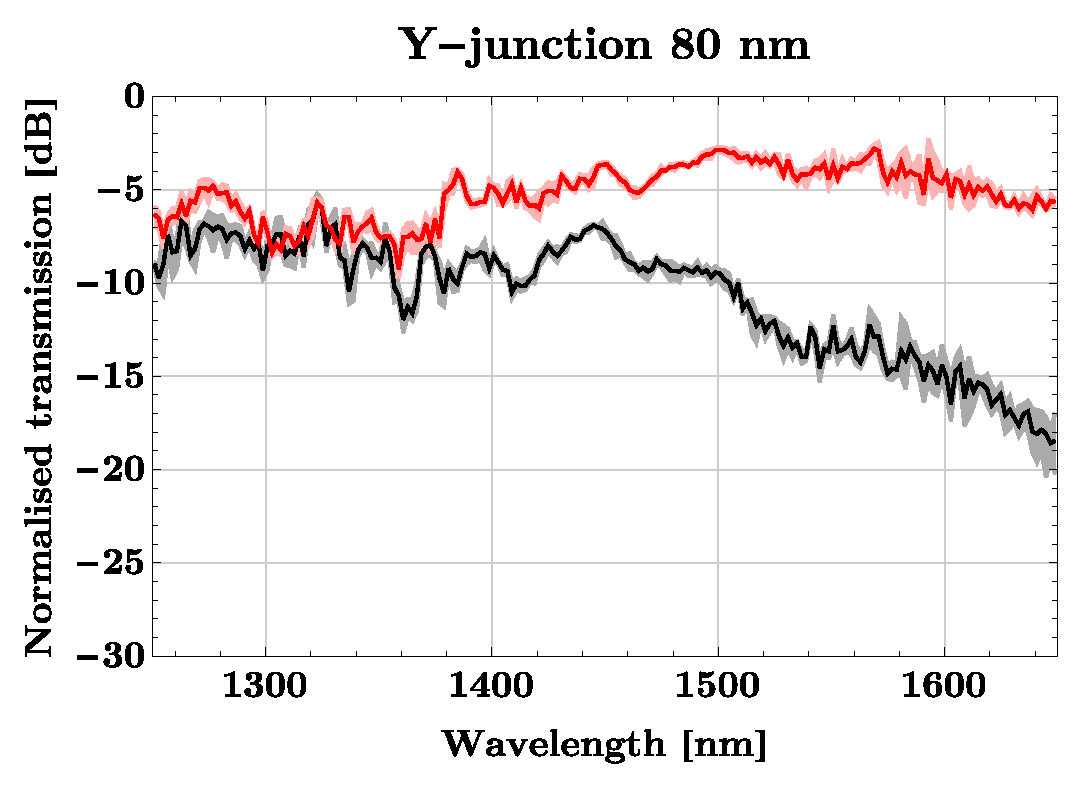
\includegraphics[width=1.0\textwidth]
        {fig/Kilde3Supercontinuum/yjunc80supercontinuum.eps}
        \caption{Transmission through the Y-junction structure with feature size 80 nm.}
    \end{subfigure}
    \caption{Normalised transmission through fabricated structures. Black: Signal through upper output waveguide. Red: signal through lower output waveguide. The shaded regions mark maximum and minimum values and are obtained through 5-blocking (See the Error Bars subsection  at page \pageref{sec:errorbars} for details). Measurements are obtained using the supercontinuum laser as a light source, see Table \ref{tablelightsources}.}
    \label{fig:transmissionkilde3}
    
\end{figure}

%The error bars mark maximum and minimum values (see the Error Bars subsection at page \pageref{sec:errorbars}) for details)